%!TEX root = ../dissertation.tex

\chapter{A brief history of GNSS}

In order to understand the context in which the problem of data authentication
for Galileo is studied, it's useful to know how the major GNSS constellations
evolved and what are the traits that characterize them at present time. In
this chapter we'll briefly introduce Galileo, GPS, and the other main players
in the satellite positioning arena.

\section{Global Positioning System (GPS)}
In February 1978, the first satellite of the Block I family was put in orbit by
the U.S. government. It was the first of a series of 11 satellites that will
constitute the prototype of what's currently known as GPS. This was the first
concrete realization of what would soon be world's most used radio navigation
system, and was the result of putting together ideas and prototypes that had
been developed by several U.S. military branches.

\subsection{Overview}
As of today, GPS is comprised of three segments: the space segment, ground
segment and user segment.

The space segment is the constellation of satellites that broadcast the radio
signal used by users to determine their positions. The ground segment is the
operating network in charge of maintaining satellites in their proper orbit and
of making sure the data that's sent is accurate. The user segment is composed of
user receiving equipment. GPS receivers are mainly responsible for resolving the
PVT equation after having acquired and tracked a sufficient number of
satellites. In addition to that, GPS receivers can also offer other kinds of
measurements - like platform attitude (heading, pitching and roll) - or function
as precise sources of time.

\subsection{Ground segment}
Fundamental to the correct operation of GPS is the health of the satellite
constellation and the accuracy of the navigation message. These two tasks are
the main responsibility of the ground segment - which includes a redundant
Master Control Station (MCS), monitoring stations (MS) and ground antennas (GA).
The MCS performs various functions like generating the navigation message,
monitoring SVs health and performing housekeeping operations on them, and
maintaining time synchronization against UTC.

In order to do so, the MCS communicates through satellites via GAs, which are
deployed across the globe so that each satellite can be reached by one to four
antennas depending on its position. A GA is a full-duplex S-band communication
facility that can hold a dedicated control and command session with a SV,
operating under control of the MCS.

To receive precise information over the constellation's health, the MCS also
operates a set of MSs that is capable of receiving GPS signal over the full
L-band and to send this signal together with meteorological data back to the
MCS. In addition to that, MSs include as part of their equipment high precision
redunant cesium clocks, which are used as a reference to measure precision of
the received data.

\subsection{Space segment}
The original design of GPS includes 24 satellites, divided in six orbital
planes positioned approximately \num{26600}\si{km} from the mass center of
Earth. The nominal orbital period is one-half of a sidereal day, or 11 hours and
58 minutes. This design allows for global coverage, meaning that at nominal
constellation operativity a minimum of three satellites is visible at any
position on Earth's surface.

Space vehicles (SVs) had undergone several modernizations steps starting from
the first launch in 1973. Subsequent developments are organized into blocks,
Block I being the first. The current constellation includes SVs from blocks IIR,
IIR-M and IIF, with a new block IIIA being planned for the next years.

Nevertheless, the main components of a SV remain the same: an antenna farm,
antennas for communication with the ground segments, a solar array for providing
energy to the satellite, a propulsion engine for orbital adjustments,
high-precision rubidium clocks, memory storage for robust operation under loss
of link with the ground segment, and of course a computing unit. Each of these
main building blocks are subject of the modernization efforts, with the goal of
making each new block more robust to adverse oribting conditions, more tolerant
to failures, more flexible to changing requirements, and more precise. At the
same time, every improvement contributes to achieve higher SV longevity: as an
example the design life of a Block I satellite was 5 years, while that of a
Block IIF satellite is 12 years.

\subsection{Signal features}
Modernization of satellites doesn't happen only because of hardware
improvements, but also because the GPS specification is in constant evolution.
The current GPS signal plan comprises transmission on three separate bands: L1,
L2 and L5. The former two bands are part of the original plan, which included a
C/A (coarse acquisition) signal on L1 and a military signal named P(Y) on both
L1 and L2. Modernization of the signal plan introduced three new civil signals,
one on L1 (L1C), one on L2 (L2C) and one on a new band L5 which will also
support SoL (Safety of Life) operations. In addition to this, a new military
signal (M) has been added on the L1 and L2 bands.

Originally, the GPS signal used a BPSK modulation that in conjunction with the
use of spreading code allowed for maximization of bandwidth usage. To accomodate
for transmission of different signals on the same frequency band, BOC modulation
has been introduced in newer signals. This achieves sufficient spectral
separation for existing receivers to keep working and for new receivers to be
able to isolate each transmission. This idea has been also a major driver in the
Galileo's signal plan as explained later in this chapter.

\section{Galileo}
Following the initiative of the U.S. government and that of the former Russian
federation, in 1998 the European Union decided to develop its own satellite
constellation to offer positioning services. Despite the challenge of being
developed as part of a program that bonds together 27 member states with
individual agendas and priorities, Galileo is set to mark a milestone in the
evolution of positioning services. Being the youngest of the global
constellations, it builds on top of the lessons learned during four decades of
GPS evolution; this reflects in the design of the signal plan and its offerings.

\subsection{Political context}
In the mid-90s the European Union started considering developing its own
satellite navigation system, with three main motivations: to increase control on
satellite-based safety-critical navigation systems, to ensure a positioning
service independent of the risk of potential U.S. policy changes to GPS
availability, and to support EU industry competitivenes in the global market of
satellite navigation.

Once defined the political scope of the project, parallel efforts were launched
to define service levels, space and ground architectures, frequency plan and
signal design. At the same time, a strong formal cooperation between EU and U.S.
resulted in the release of a framework to achieve full interoperability and
radio frequency compatibility between Galileo and GPS.

\subsection{Service offering}
Similarly to GPS, Galileo's signal plan is intended to offer open civil access
as well as access restricted to authorized users. Differently than GPS though,
the service plan for Galileo includes from the start a broader range of options:
\begin{itemize}
  \item \textbf{Open Service} provides positioning and timing information
    worldwide, and is meant to be accessible free of charge from any user
    equpped with a Galileo compatible navigation receiver. This is similar to
    the service level of GPS L1 C/A, L2C or L5
  \item \textbf{Public Regulated Service} provides the same capabilities as the
    Open Service signal, but it's meant to be restricted to only
    government-authorized users, for use in sensitive applications. This is
    similar to the service level of GPS P(Y) or M codes
  \item \textbf{Commercial Service} is included in the current service
    specification but its definition is as of now undergoing. The idea for
    the CS is to offer "added value" with respect to the Open Service, mainly in
    terms of high accuracy and authentication. In addition, this service is
    going to provide the possibility of globally transmitting external data in
    real-time. This service offering is completely new in the GNSS landscape and
    has currently no similar counterpart in other constellations
  \item \textbf{Search and Rescue} is meant to enhance the current capability of
    another system, namely LEOSAR, for use in assistance of users in distress.
    Through SAR users that need assistance can transmit a beacon signal that can
    be received by Galileo satellites and then relayed to ground stations
    that can then proceed with locating the source of the beacon by reversing
    the PVT equation normally used in GNSS
  \item \textbf{Safety of Life} is a service aimed at offering worldwide system
    integrity. It has been foreseen by the Galileo program but it's actual
    implementation has been postponed to later phases
\end{itemize}
Each of these services is going to be available on one or more frequencies of
Galileo's signal plan, which is described next.

\subsection{Signal plan}
The Galileo signal is in general very similar to that of GPS, in the sense that
in most general terms it's composed of the sum of a PRN spreading code and a
navigation message. Some peculiar characteristics set the Galileo signals apart
from the GPS ones.

The main difference is that the PRN codes employed in Galileo are not pure Gold
codes as in the case of GPS, but have been developed with genetic algorithms
starting from such standard codes. Each spreading code is generated by the sum
of a primary and a secondary code. Some of the primary codes can be generated
using LFSR, but most of them need to be stored in memory. The secondary codes
are 2 to 3 orders of magnitude shorter than the primary codes, and can be easily
stored in a few memory words. The reason for this tradeoff is that Galileo codes
are heavily optimized for their cross-correlation properties and interference
mitigation capabilities.

On the other hand the navigation message is of three different kinds, depending
on the band of transmission and on the service level. For OS, two types of
message are available: F/NAV and I/NAV. For CS, I/NAV and C/NAV, the C/NAV being
encrypted and not covered within the public ICD. The main difference between
these messages is the length of the transmitted pages, which is bound to the
chip rate of the signal they're transmitted on. In general, though, each of them
conforms to a general navigation message structure.  Independently from its
length, the navigation message is composed of a repetition of frames which share
the same structure. Each frame is composed of a number of sub-frames, which are
in turn composed of a number of pages. Pages can be of different type, which is
identified in a dedicated field. Each page type contains different sets of
information. In general though, Galileo navigation message contains three main
types of information:
\begin{itemize}
  \item Ephemeris: characterize the orbit of each satellite, allowing users to
    calculate its coordinates in a Earth Centered, Earth Fixed (ECEF) reference
    frame
  \item Time information: such as GST, clock correction, GST-UTC and GST-GPS
    conversion parameters
  \item Ionospheric correction: a set of parameters that allow receivers to
    adjust the PVT equation to account for ionospheric interference
\end{itemize}

\vspace{\baselineskip}

Galileo signals are transmitted over four bands within the official RNSS and
ARNS frequency bands. These four bands are named E1, E5a, E5b and E6. The center
frequency of these bands ranges from \num{1176.450} \si{MHz} to \num{1575.420}
\si{MHz}, while the transmitted bandwidth ranges between \num{20.460} \si{MHz}
and \num{51.150} \si{MHz}. A full account of the frequency allocation and
bandwidth distribution is provided in figure ~\ref{fig:galileo_frequencies} and
table ~\ref{table:galileo_signals}.

\begin{figure}[h!]
  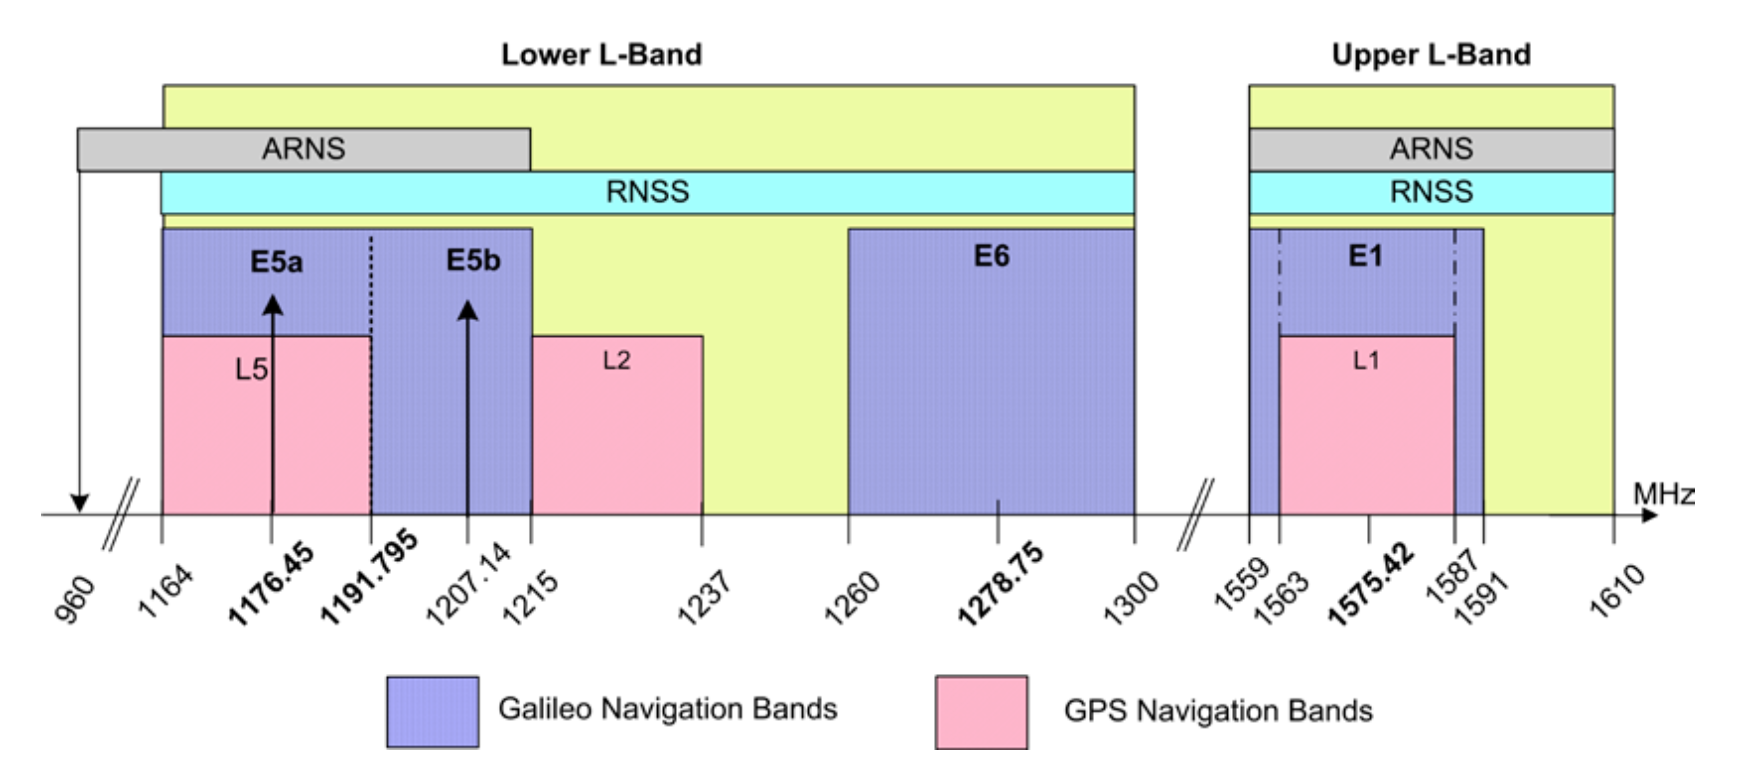
\includegraphics[width=\linewidth]{figures/galileo_signal_plan.png}
  \caption{Galileo and GPS frequency spectrum}
  \label{fig:galileo_frequencies}
\end{figure}

\begin{longtable}[]{@{}ll@{}}
  \toprule
  Signal & Carrier Frequency (MHz)\tabularnewline
  \midrule
  \endhead
  E1 & 1575.420\tabularnewline
  E6 & 1278.750\tabularnewline
  E5 & 1191.795\tabularnewline
  E5a & 1176.450\tabularnewline
  E5b & 1207.140\tabularnewline
  \bottomrule
  \caption{Galileo signal plan}
  \label{table:galileo_signals}
\end{longtable}

All Galileo signals are RHCP, and independently from the modulation are composed
of in-phase and quadrature components. In-phase components carry the navigation
message, while quadrature components only carry the PRN code with no data; such
pilot signal has the purpose of aiding initial signal acquisition.

As in the case of GPS, usage of PRN allows for transmission of multiple signals
from different SVs over the same frequency - an implementation of Direct
Sequence Spread Spectrum Code Division Multiple Access (DS-SS CDMA). Apart from
that, Galileo employs a BOC modulation to allow for interoperation with the GPS
signal, as for example in the case of L1/E1 the same frequency band is used by
the two system. The topic of interoperability is expanded in a following
section.

Looking at the signal plan, one might notice that Galileo transmits a variety of
signals much larger than the current GPS one. This variety is characterized by
variations in the code length and navigation message data rate. This is an
engeenering design choice to support a wide variety of use cases, such as users
that receive a very faint signal, rather than users that move at high speed.

\subsection{System architecture}
Transmission and control of the described range of signals is performed within
Galileo's system infrastructure, which is composed of three major blocks: the
Core Infrastructure, Service Facilities and Support Facilities.

Galileo's Service Facilities provide steering corrections to the CI by
monitoring the alignment of time and reference geodetic model with the
international meteorological standard (UTC and ITRF, respectively).

Galileo's Support Facilities are not directly involved in the routine provision
of services but play a major role in the deployment, testing and subsequent
control of satellites into orbit.

Galileo's CI is instead the main part of the system infrastructure and can be
subsequently divided in three main segments: Galileo's Space Segment, Ground
Control Segment and Ground Mission Segment.

The Space Segment, as defined in the reference constellation, is composed of 24
operative satellites distributed in 3 circular orbits with a radius of 29,600 km
and an orbital period of approximately 14h. At the time of writing, information
on the actual Galileo constellation can be found in \cite{galileo_constellation}.

Galileo's satellites are currently divided in four families: Giove-A and Giove-B
are the initial prototypes and have been used for the initial testing phase;
their designed lifetime is of 27 months. Currently being deployed is the IOV
family, with improved design and a projected lifetime of 12 years; these
satellites are used for the In-Orbit Validation phase of the project. Similar to
the IOV satellites are those in the last family, namely FOC; these are meant to
support Galileo's Full Operational Capability and has been deployed starting
from Q3 2014. In terms of functionalities, overall budget envelope and
performances these last two families are close to each other.

The constellation is managed during normal system operation by the GCS, which is
composed of two kind of facilities: control centers (GCC) and telemetry stations
(TT\&C). \\
The GCCs perform duties related to monitoring and control of the
constellation, together with planning, flight dynamics and operations
preparation of the same.\\
Through TT\&C, instead, ground control performs data exchange with the entire
constellation through 11m antenna dishes that operates in the S-band. Normally
these stations are used to perform tele-command of the satellites and to receive
telemetry data that is further used for off-line satellite orbit determination.

The signal sent to the user by spacecrafts is generated by the GMS, a network of
sensor stations, control centers and up-link stations that interoperate to
perform a distinct set of operations:
\begin{itemize}
  \item generation and distribution of Galileo System Time (GST) to satellites
    and ground segments
  \item generation and distribution of Galileo OS and PRS navigation messages
  \item distribution of mission data provided by Galileo Service Facilities for
    CS and SAR signals
  \item provision of the physical interface with the US Naval Observatory for
    generation of the GPS Galileo interoperability products like the GPS to
    Galileo time offset
\end{itemize}

\section{Other constellations}
In the GNSS panorama, there are two other constellations worth of note for the
role they're playing or will predictbly play in shaping up the future of a
common GNSS infrastructure: Russian GLONASS and Chinese BeiDou.

\subsection{GLONASS}
With a history similar to that of GPS, the GLONASS program was initiated in the
1970s to support military requirements. Later on, early tests demonstrated the
possibility of handling also civilian use. The first launch dates back to 1982.
Despite having caused interference within the radio astronomy observation band,
development of the program continued steadily - even past the demise of the
Soviet Union. In 1995 the last batch of satellites was launched to complete the
constellation, which nominally consisted of 24 satellites. Shortly after,
however, a number of older satellites failed and the Russians failed to
replenish the constellation. In 2001, restoration of the degraded constellation
was made a top government priority; since 2011 GLONASS is again fully
operational with global availability.

\vspace{\baselineskip}

GLONASS constellation consists of 24 satellites, 21 of which fully operative and
3 acting as spares. The satellites are organized in 3 orbital planes \ang{120}
apart from each other in right ascension with a period of 11 hours and 15
minutes.

Such configuration provides continuous visibility of no less than 4 satellites
to over 97\% of Earth's surface. A full 24 satellite configuration would instead
provide continuous visibility of no less than 5 satellites to more than 99\% of
the Earth's surface.

\vspace{\baselineskip}

Differently than other systems, GLONASS historically used FDMA as a multiplexing
technique, which increases complexity on the receiver side but allows for better
interference rejection properties. As of 2016, a new ICD was published
containing new CDMA signals, namely three open (L1OC, L2OC and L3OC) and two
restricted (L1SC and L2SC).

The older FDMA signals are transmitted on a different frequency by each
satellite in the L1 and L2 bands, following the equation
\begin{equation}
  \begin{array}{l}
    f_{K1} = f_{01} + K \Delta f_1, \\
    f_{K2} = f_{02} + K \Delta f_2
  \end{array}
\end{equation}

where

\begin{equation}
  \begin{array}{l}
    f_{01} = 1602 MHz, \Delta f_1 = 562.5 kHz \\
    f_{02} = 1246 MHz, \Delta f_2 = 437.5 KHz
  \end{array}
\end{equation}

To avoid interference with the radio astronomy band, the value of $K$ changes
between satellites in a range that goes from -7 to 4. To account for just 12
different available frequencies, antipodal satellites are going to transmit on
the same frequency (i.e. will share the same value of $K$). Since these
satellite pairs are on opposite sides of Earth's surface, users are not
impacted.

GLONASS signal is of two types: C/A code or P code. The latter is restricted to
military use, while the former is open for civilian use. Both signal types
transmit a navigation message with a rate of 50 bps. Also, both signals are
composed by a PRN code message and a navigation message. The main content of the
navigation message is represented by the ephemeris, but in addition to that
GLONASS transmits other data such as epoch timing, synchronization bits,
satellite health and age of data fields. Each transmission contains accurate
ephemeris information for the transmitting satellite and approximate (i.e.
almanac) information about all the satellites in the constellation.

\subsection{BeiDou}
Another global player in radio navigation satellite systems comes from China
under the name of BeiDou. The initial concept was developed in the 1980s, and
the first launch of an experimental satellite happened in the year 2000. In
2007, the first version of BeiDou (BeiDou-1) became fully operative with a
regional coverage of China and the surrounding countries.

As of mid-2007, deployment of the BeiDou-2 system began with an expected
timeline lasting till 2020, which will bring BeiDou-2 at full operativity and
global coverage. This will consist of 35 satellites, organized in different
group. 5 satellites will be on geostationary orbit; 3 of them will be on
inclined geosynchronous orbit; finally, 27 of them will be displaced in 3 medium
Earth orbits.

BeiDou-2 will transmit on 5 bands: E1, E2, E5B and E6. The system will transmit
two types of signal: a free service for civilian use and a restricted one for
military and government use. The free service is claimed to have location
accuracy of \num{10}\si{m}, time accuracy of \num{10}\si{ns} and velocity
accuracy of \num{0.2}\si{m/s}. The military service instead will have a location
accuracy of \num{0.1}\si{m}. The modulation of these signals uses CDMA
techniques similar to that of Galileo; the chipping rate and the data rate are
also comparable if not identical to that of Galileo OS.

Although little is known about the actual structure of the system and the
service levels to be offered, it's clear that the Chinese government is aiming
at becoming more than competitive in the arena of radio navigation systems. The
speed at which the Chinese deployed satellites in the past years hints at the
idea that BeiDou-2 will be soon an equal alternative to GPS and Galileo.

\section{Interoperability challenges}
As the number of global systems increases, and as the radio spectrum gets more
and more crowded, the problem of interoperability (or, put in different terms,
that of interference) becomes more and more relevant. In general, a choice has
to be made: should system be independent and completely isolate, or should their
design be aware of the presence of other navigation systems?

The answer came during the third meeting of of the Providers' Forum of the
International Committee on Global Navigation Satellite Systems (ICG) in 2008.
Here it was agreed that at a minimum all GNSS signals and services should be
compatible. At the same time, to the maximum extent possible open signals and
services should also be interoperable, in order to maximize benefit to all GNSS
users.

In the same committee, a contextual definition of the two terms was provided:
\begin{itemize}
  \item \textbf{Interoperability} refers to the capability for all the systems
    to be used together to provide better capabilities at the user level than
    each individual system, at a minimal additional receiver cost or complexity
  \item \textbf{Compatibility} means that two systems can be used individually
    or together with no unacceptable interference or other harm to the other
    system. For this the ITU provides a framework for discussions on
    radiofrequency compatibility.
\end{itemize}

\vspace{\baselineskip}

This formal agreement resulted in a number of significant decision in the
evolution of the design of all major GNSS.

For example, when designing the frequency plan of Galileo, one of the drivers
was the selection of common center frequencies for some of the signals: this was
to prevent unnecessary increase in the cost of multi-frquency receivers and to
make combined processing of phase observations possible.

From the point of view of signal spreading modulation, the choice of CDMA was a
significant step in the design of interoperable systems. On the same topic,
while the initial definition of GLONASS used FDMA, new signals are being
included that use CDMA.

At the data level, two other notable examples are the choice of the coordinate
reference frame and that of time reference. In particular, the Galileo
Terrestrial Reference Frame and the GPS coordinate frame (WGS84) differ a few
centimeters from the International Terrestrial Reference Frame, hence making the
two interoperable for most applications. In the case of time, both GST and GPS
time are different real-time realizations of UTC, and the service providers have
agreed to broadcast the time offset between the two standards.

The question of interoperability and compatibility has had repercussions also on
the organizational and political level. Although later unsatisfied by the role
in the project, China signed in 2004 an agreement on the cooperation in the
Galileo program between the "Galileo Joint Undertaking" and the "National Remote
Sensing of China", which resulted in 11 cooperations projects being signed
within the program between China and EU in 2006.

\section{The future of GNSS}
% TODO take inspiration from "Multi Frequency Multi Systems Receivers of
% Tomorrow" from Galileo Positioning Technology
